\documentclass[10pt,ignorenonframetext,,aspectratio=149]{beamer}
\setbeamertemplate{caption}[numbered]
\setbeamertemplate{caption label separator}{: }
\setbeamercolor{caption name}{fg=normal text.fg}
\usepackage{lmodern}
\usepackage{amssymb,amsmath}
\usepackage{ifxetex,ifluatex}
\usepackage{fixltx2e} % provides \textsubscript
\ifnum 0\ifxetex 1\fi\ifluatex 1\fi=0 % if pdftex
  \usepackage[T1]{fontenc}
  \usepackage[utf8]{inputenc}
\else % if luatex or xelatex
  \ifxetex
    \usepackage{mathspec}
  \else
    \usepackage{fontspec}
  \fi
  \defaultfontfeatures{Ligatures=TeX,Scale=MatchLowercase}
  \newcommand{\euro}{€}
\fi
% use upquote if available, for straight quotes in verbatim environments
\IfFileExists{upquote.sty}{\usepackage{upquote}}{}
% use microtype if available
\IfFileExists{microtype.sty}{%
\usepackage{microtype}
\UseMicrotypeSet[protrusion]{basicmath} % disable protrusion for tt fonts
}{}

% Comment these out if you don't want a slide with just the
% part/section/subsection/subsubsection title:
\AtBeginPart{
  \let\insertpartnumber\relax
  \let\partname\relax
  \frame{\partpage}
}
\AtBeginSection{
  \let\insertsectionnumber\relax
  \let\sectionname\relax
  \frame{\sectionpage}
}
\AtBeginSubsection{
  \let\insertsubsectionnumber\relax
  \let\subsectionname\relax
  \frame{\subsectionpage}
}

\setlength{\emergencystretch}{3em}  % prevent overfull lines
\providecommand{\tightlist}{%
  \setlength{\itemsep}{0pt}\setlength{\parskip}{0pt}}
\setcounter{secnumdepth}{0}

\title{Finance 6470 - Derivatives Markets}
\subtitle{Chapter 1 - Introduction to Derivatives}
\author{Tyler J. Brough}
\date{}

%% Here's everything I added.
%%--------------------------

\usepackage{graphicx}
\usepackage{rotating}
%\setbeamertemplate{caption}[numbered]
\usepackage{hyperref}
\usepackage{caption}
\usepackage[normalem]{ulem}
%\mode<presentation>
\usepackage{wasysym}
%\usepackage{amsmath}


% Get rid of navigation symbols.
%-------------------------------
\setbeamertemplate{navigation symbols}{}

% Optional institute tags and titlegraphic.
% Do feel free to change the titlegraphic if you don't want it as a Markdown field.
%----------------------------------------------------------------------------------
\institute{Department of Finance and Economics}

% \titlegraphic{\includegraphics[width=0.3\paperwidth]{\string~/Dropbox/teaching/clemson-academic.png}} % <-- if you want to know what this looks like without it as a Markdown field. 
% -----------------------------------------------------------------------------------------------------
\titlegraphic{
\includegraphics[width=0.3\paperwidth]{\string~./images/vertical-logo-blue.png}}

% Some additional title page adjustments.
%----------------------------------------
\setbeamertemplate{title page}[empty]
%\date{}
\setbeamerfont{subtitle}{size=\small}

\setbeamercovered{transparent}

% Some optional colors. Change or add as you see fit.
%---------------------------------------------------
\definecolor{clemsonpurple}{HTML}{522D80}
% \definecolor{clemsonorange}{HTML}{EA6A20}
 \definecolor{clemsonorange}{HTML}{F66733}
\definecolor{uiucblue}{HTML}{003C7D}
\definecolor{uiucorange}{HTML}{F47F24}
%\definecolor{usublue}{HTML}{2D3280}
%\definecolor{usublue}{HTML}{000066}
%\definecolor{usublue}{HTML}{273849}
%\definecolor{usublue}{HTML}{78281F}
%\definecolor{usublue}{HTML}{A04000}


%\definecolor{usublue}{HTML}{3498DB}
%\definecolor{bluegray}{HTML}{334760}
\definecolor{usublue}{HTML}{C0392B}
\definecolor{bluegray}{HTML}{34495E}

\definecolor{gray}{HTML}{446280}

% Some optional color adjustments to Beamer. Change as you see fit.
%------------------------------------------------------------------
%\setbeamercolor{frametitle}{fg=clemsonpurple,bg=white}
\setbeamercolor{frametitle}{fg=usublue,bg=white}
\setbeamercolor{title}{fg=usublue,bg=white}
\setbeamercolor{local structure}{fg=usublue}
\setbeamercolor{section in toc}{fg=usublue,bg=white}
% \setbeamercolor{subsection in toc}{fg=clemsonorange,bg=white}
\setbeamercolor{footline}{fg=usublue!50, bg=white}
\setbeamercolor{block title}{fg=gray,bg=white}


\let\Tiny=\tiny


% Sections and subsections should not get their own damn slide.
%--------------------------------------------------------------
\AtBeginPart{}
\AtBeginSection{}
\AtBeginSubsection{}
\AtBeginSubsubsection{}

% Suppress some of Markdown's weird default vertical spacing.
%------------------------------------------------------------
\setlength{\emergencystretch}{0em}  % prevent overfull lines
\setlength{\parskip}{0pt}


% Allow for those simple two-tone footlines I like. 
% Edit the colors as you see fit.
%--------------------------------------------------
\defbeamertemplate*{footline}{my footline}{%
    \ifnum\insertpagenumber=1
    \hbox{%
        \begin{beamercolorbox}[wd=\paperwidth,ht=.8ex,dp=1ex,center]{}%
      % empty environment to raise height
        \end{beamercolorbox}%
    }%
    \vskip0pt%
    \else%
        \Tiny{%
            \hfill%
		\vspace*{1pt}%
            \insertframenumber/\inserttotalframenumber \hspace*{0.1cm}%
            \newline%
            \color{usublue}{\rule{\paperwidth}{0.4mm}}\newline%
            \color{bluegray}{\rule{\paperwidth}{.4mm}}%
        }%
    \fi%
}

% Various cosmetic things, though I must confess I forget what exactly these do and why I included them.
%-------------------------------------------------------------------------------------------------------
\setbeamercolor{structure}{fg=blue}
\setbeamercolor{local structure}{parent=structure}
\setbeamercolor{item projected}{parent=item,use=item,fg=usublue,bg=white}
\setbeamercolor{enumerate item}{parent=item}

% Adjust some item elements. More cosmetic things.
%-------------------------------------------------
\setbeamertemplate{itemize item}{\color{usublue}$\bullet$}
\setbeamertemplate{itemize subitem}{\color{usublue}\scriptsize{$\bullet$}}
\setbeamertemplate{itemize/enumerate body end}{\vspace{.6\baselineskip}} % So I'm less inclined to use \medskip and \bigskip in Markdown.

% Automatically center images
% ---------------------------
% Note: this is for ![](image.png) images
% Use "fig.align = "center" for R chunks

\usepackage{etoolbox}

\AtBeginDocument{%
  \letcs\oig{@orig\string\includegraphics}%
  \renewcommand<>\includegraphics[2][]{%
    \only#3{%
      {\centering\oig[{#1}]{#2}\par}%
    }%
  }%
}

% I think I've moved to xelatex now. Here's some stuff for that.
% --------------------------------------------------------------
% I could customize/generalize this more but the truth is it works for my circumstances.

\ifxetex
\setbeamerfont{title}{family=\fontspec{serif}}
\setbeamerfont{frametitle}{family=\fontspec{serif}}
\usepackage[font=small,skip=0pt]{caption}
 \else
 \fi

% Okay, and begin the actual document...

\begin{document}
\frame{\titlepage}

\begin{frame}
\section{Chapter 1: Introduction to Derivatives}
\end{frame}

\begin{frame}{What is a Derivative?}
\protect\hypertarget{what-is-a-derivative}{}
\begin{itemize}
\item
  \textbf{Definition:} a financial instrument that has a value
  determined by the price of something else
\item
  An agreement where you pay \(\$1\) if the price of corn is greater
  than \(\$3\) and receive \(\$1\) if the price of corn is less than
  \(\$1\) is a derivative

  \begin{itemize}
  \tightlist
  \item
    This contract can be used to speculate on the price of corn or it
    can be used to reduce risk. It is not the contract itself, but how
    it used, and who uses it, that determines whether or not it is
    risk-reducing.
  \end{itemize}
\end{itemize}
\end{frame}

\begin{frame}{An Overview of Financial Markets}
\protect\hypertarget{an-overview-of-financial-markets}{}
The trading of a financial asset involves at least four discrete steps:

\begin{itemize}
\item
  A buyer and a sellter must locate one another and agree on a price
\item
  The trade must be \emph{cleared} (the obligations of each party are
  specified)
\item
  The trade must be \emph{settled} (the buyer and the seller must
  deliver the cash or securities necessary to satisfy their obligations
  in the required period of time)
\item
  Ownership records are updated
\end{itemize}

\vspace{3mm}

\textbf{\emph{NB:}} notice that well-defined property rights are an
assumption of properly functioning capital markets.
\end{frame}

\begin{frame}{An Overview of Financial Markets (Continued)}
\protect\hypertarget{an-overview-of-financial-markets-continued}{}
\begin{itemize}
\item
  Much trading of financial claims takes place on organized exchanges.
  In the past, the exchange was solely a physical location where traders
  would buy and sell. Such in-person venues have largely been replaced
  by electronic networks that provide a virtual trading venue.
\item
  After a trade has taken place, a \textbf{clearinghouse} matches the
  buyers and sellers, keeping track of their obligations and payments.
  To facilitate these payments and to help manage credit risk, a
  derivatives clearinghouse typically imposes itself in the transaction,
  becoming the buyer to all sellers and the seller to all buyers.
\end{itemize}
\end{frame}

\begin{frame}{An Overview of Financial Markets (Continued)}
\protect\hypertarget{an-overview-of-financial-markets-continued-1}{}
\begin{itemize}
\item
  It is possible for large traders to trade many financial claims
  directly with a dealer bypassing organized exchanges. Such trading is
  said to occur in the \textbf{over-the-counter} (OTC) market
\item
  Exchange activity is public and highly regulated
\item
  OTC trading is not easy to observe or measure and is generally less
  regulated
\item
  For many categories of financial claims, the value of OTC trading is
  greater than the value traded on exchanges.
\end{itemize}
\end{frame}

\begin{frame}{An Overview of Financial Markets (Continued)}
\protect\hypertarget{an-overview-of-financial-markets-continued-2}{}
There are at least four different measures of a market and its activity

\begin{itemize}
\item
  \textbf{Trading volume}. This measure counts the number of financial
  claims that change hands
\item
  \textbf{Market value}. The market value is the sum of the market value
  of the claims that \emph{could} be traded, without regard to whether
  they have traded
\item
  \textbf{Notional value}. Notional value measure the \emph{scale} of a
  position, usually with reference to some underlying asset
\item
  \textbf{Open Interest}. Open interest measures the total number of
  contracts for which counterparties have a future obligation to perform
\end{itemize}
\end{frame}

\begin{frame}{Derivatives Markets}
\protect\hypertarget{derivatives-markets}{}
The introduction of derivatives markets in a market often coincides with
an increase in price risk in that market

\begin{itemize}
\item
  Currencies were permitted to float in 1971 when the gold standard was
  officially abandoned. The modern market in financial derivatives
  begain in 1972, when the Chicago Mercantile Exchange started trading
  futures contracts on seven currencies.
\item
  OPEC's 1973 reduction in the supply of oil was followed by high and
  variable oil prices
\item
  U.S. interest rates became more volatile following inflation and
  recessions in the 1970s
\item
  The market for natural gas has been deregulated gradually since 1978,
  resulting in a volatile market in recent years
\item
  The deregulation of electricity began during the 1990s
\end{itemize}
\end{frame}

\begin{frame}{Increased Volatility \ldots{}}
\protect\hypertarget{increased-volatility}{}
\begin{itemize}
\tightlist
\item
  Oil prices 1947-2011
\end{itemize}

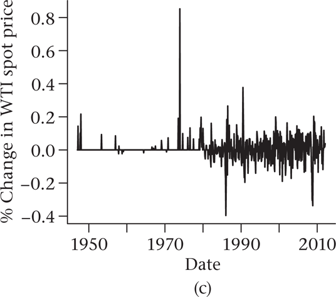
\includegraphics[scale=0.3]{./images/Picture1.png}

\vspace{5mm}

\begin{itemize}
\tightlist
\item
  Dollar/Euro rate 1947-2011
\end{itemize}

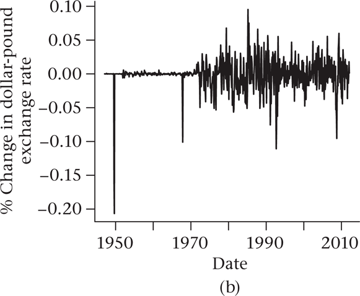
\includegraphics[scale=0.3]{./images/Picture2.png}
\end{frame}

\begin{frame}{\ldots{} Led to New and Big Markets}
\protect\hypertarget{led-to-new-and-big-markets}{}
\begin{itemize}
\tightlist
\item
  Exchange-traded derivatives
\end{itemize}

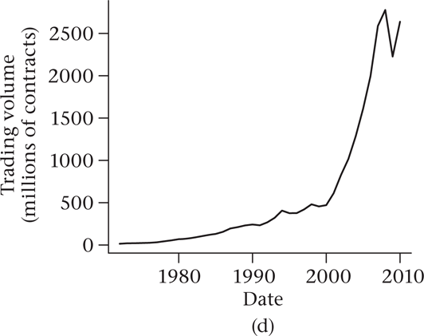
\includegraphics[scale=0.5]{./images/Picture7.png}

\begin{itemize}
\tightlist
\item
  Over-the-counter markets have also grown rapidly over this period
\end{itemize}
\end{frame}

\begin{frame}{Exchange Traded Contracts}
\protect\hypertarget{exchange-traded-contracts}{}
Contracts proliferated in the last four decades

\vspace{3mm}

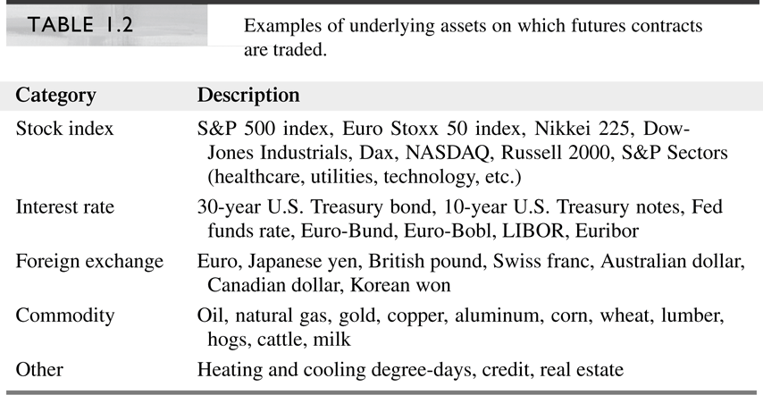
\includegraphics[width=0.7\textwidth]{./images/Picture3.png}
\end{frame}

\begin{frame}{The Role of Financial Markets}
\protect\hypertarget{the-role-of-financial-markets}{}
\begin{itemize}
\item
  Insurance companies and individual communities/families have
  traditionally helped each other to share risks
\item
  Markets make risk-sharing more efficient

  \begin{itemize}
  \tightlist
  \item
    Diversifiable risks vanish
  \item
    Non-diversifiable risks are reallocated to those most willing to
    hold it
  \end{itemize}
\end{itemize}
\end{frame}

\begin{frame}{The Uses of Derivatives}
\protect\hypertarget{the-uses-of-derivatives}{}
(Some) Uses for derivative contracts

\begin{itemize}
\item
  \textbf{Risk management}. Derivatives are a tool for companies and
  other users to reduce risks
\item
  \textbf{Speculation}. Derivatives can serve as investment vehicles
\item
  \textbf{Reduce transaction costs}. Sometimes derivatives provide a
  lower cost way to undertake a particular financial transaction
\item
  \textbf{Regulatory arbitrage}. It is sometimes possible to circumvent
  regulatory restrictions, taxes, and accounting rules by trading
  derivatives
\end{itemize}
\end{frame}

\begin{frame}{Perspectives on Derivatives}
\protect\hypertarget{perspectives-on-derivatives}{}
\begin{itemize}
\tightlist
\item
  End users

  \begin{itemize}
  \tightlist
  \item
    Corporations
  \item
    Investment managers
  \item
    Investors
  \end{itemize}
\item
  Intermediaries

  \begin{itemize}
  \tightlist
  \item
    Market-makers
  \item
    Traders
  \end{itemize}
\item
  Economic observers

  \begin{itemize}
  \tightlist
  \item
    Regulators
  \item
    Researchers
  \end{itemize}
\end{itemize}
\end{frame}

\begin{frame}{Financial Engineering and Security Design}
\protect\hypertarget{financial-engineering-and-security-design}{}
\begin{itemize}
\item
  The construction of a financial product from other products
\item
  New securities can be designed by using existing securities
\item
  Financial engineering principles

  \begin{itemize}
  \tightlist
  \item
    Facilitate hedging of existing positions
  \item
    Allow for creation of customized products
  \item
    Enable understanding of complex positions
  \item
    Render regulation less effective
  \end{itemize}
\end{itemize}
\end{frame}

\begin{frame}{Transaction Costs and the Bid-Ask Spread}
\protect\hypertarget{transaction-costs-and-the-bid-ask-spread}{}
\begin{itemize}
\tightlist
\item
  Buying and selling a financial asset

  \begin{itemize}
  \tightlist
  \item
    Brokers: commissions
  \item
    Market-makers: bid-ask (offer) spread
  \end{itemize}
\item
  Example 1.1: Buy and sell 100 shares of XYZ

  \begin{itemize}
  \tightlist
  \item
    XYZ: bid \(= \$49.75\), offer \(= \$50\), commission \(= \$15\)
  \item
    Buy: \((100 \times \$50) + \$15 = \$5,015\)
  \item
    Sell: \((100 \times \$49.75) - \$15 = \$4,960\)
  \item
    Transaction cost: \(\$5,015 - \$4,960 = \$55\)
  \end{itemize}
\end{itemize}
\end{frame}

\begin{frame}{Short-Selling}
\protect\hypertarget{short-selling}{}
\begin{itemize}
\tightlist
\item
  When the price of an asset is expected to fall

  \begin{itemize}
  \tightlist
  \item
    First: borrow and sell an asset (get \(\$\$\))
  \item
    Then: buy back and return the asset (pay \(\$\))
  \item
    If price fell in the mean time: Profit \(\$ = \$\$ - \$\)
  \item
    The lender must be compensated for dividends received (lease-rate)
  \end{itemize}
\item
  Example: short-sell IBM stock for 90 days
\end{itemize}

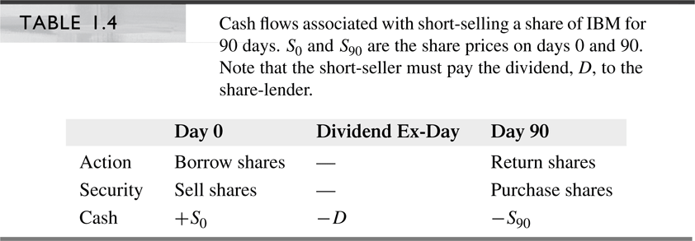
\includegraphics[width=0.7\textwidth]{./images/Picture4.png}
\end{frame}

\begin{frame}{Short-Selling (Continued)}
\protect\hypertarget{short-selling-continued}{}
\begin{itemize}
\tightlist
\item
  Why short-sell?

  \begin{itemize}
  \tightlist
  \item
    Speculation
  \item
    Financing
  \item
    Hedging
  \end{itemize}
\item
  Credit risk in short-selling

  \begin{itemize}
  \tightlist
  \item
    Collateral and ``haircut''
  \end{itemize}
\item
  Interest received from lender on collateral

  \begin{itemize}
  \tightlist
  \item
    Scarcity decreases the interest rate
  \item
    Repo rate in bond markets
  \item
    Short rebate in the stock market
  \end{itemize}
\end{itemize}
\end{frame}

\begin{frame}{}
\protect\hypertarget{section}{}
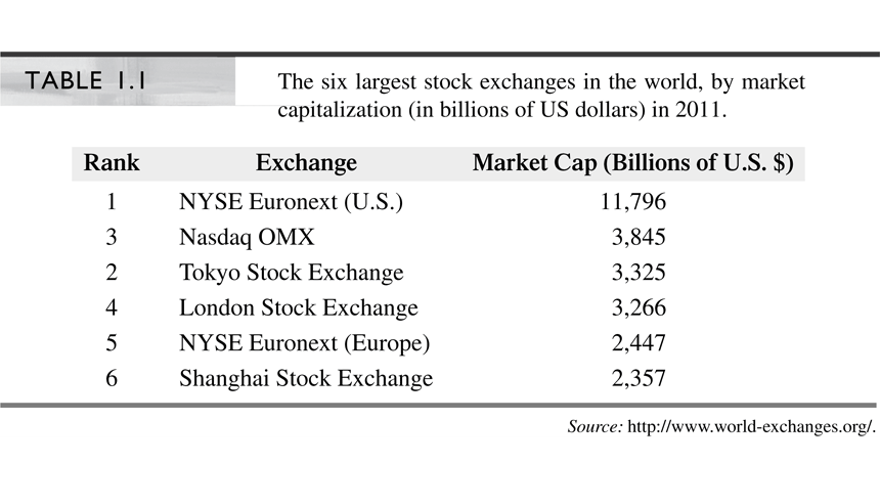
\includegraphics[width=\textwidth]{./images/Picture5.png}
\end{frame}

\begin{frame}{}
\protect\hypertarget{section-1}{}
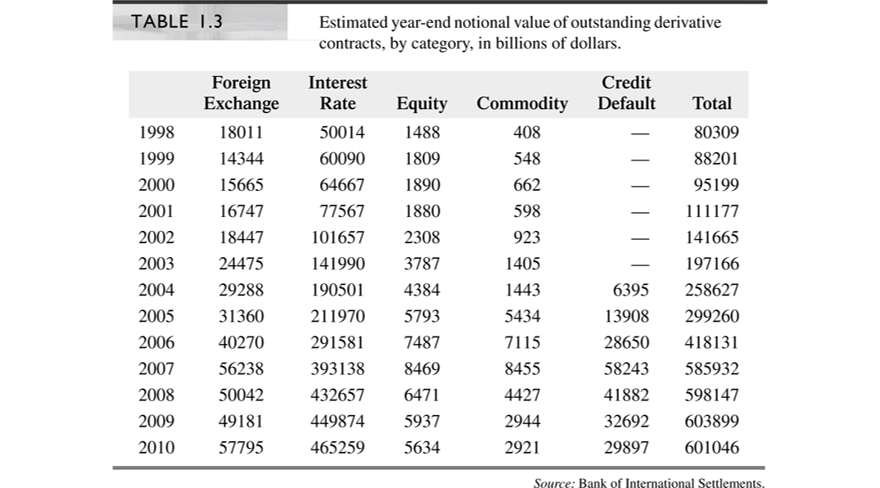
\includegraphics[width=\textwidth]{./images/Picture6.png}
\end{frame}


%\section[]{}
%\frame{\small \frametitle{Table of Contents}
%\tableofcontents}
\end{document}
